\section*{Výsledky měření}
Měření proběhlo při normálním tlaku a pokojové teplotě (přibližně \SI{22}{\degreeCelsius}).
Všechny uvedené nejistoty jsou standardní a v zápisu \num{10(1)} znamená číslo v závorce nejistotu v řádu poslední uvedené číslice.

Měřili jsme tři feritové kroužky označené římskými I, II, III.
Jejich vlastnosti jsou uvedeny v tabulce \ref{t:krouzky}.

\begin{tabulka}[htbp]
\centering
\begin{tabular}{c|c|c|c|c|c}
kroužek & $n_1$ & $n_2$ & $d_1$ & $d_2$ & $v$ \\ \hline
I & \num{50} & \num{6} & \SI{29.20}{\mm} & \SI{20.75}{\mm} & \SI{4.40}{\mm} \\
II & \num{50} & \num{6} & \SI{30.65}{\mm} & \SI{21.80}{\mm} & \SI{4.35}{\mm} \\
III & \num{300} & \num{6} & \SI{31.00}{\mm} & \SI{21.80}{\mm} & \SI{4.15}{\mm} \\
\end{tabular}
\caption{Měřené feritové kroužky}
\label{t:krouzky}
\end{tabulka}

Proud i napětí jsme měřili multimetrem METEX M-3720D.

Při kalibraci jsme používali střídavé napětí o síťové frekvenci \SI{50}{\hertz}, proto $\omega = 2\pi\cdot\SI{50}{\radian\per\second}$.

Nastavili jsme napětí na normálu takové, aby úsečka na osciloskopu byla vysoká jako hysterezní smyčka každého kroužku při nejvyšším měřeném proudu.
Pro kroužky I a III ukazoval voltmetr napětí \SI{7.0(1)}{\volt} a pro kroužek II \SI{5.7(1)}{\volt}.
Napětí $U_{ef}$ je tedy rovné tisícině této hodnoty.

Podle \eqref{e:kalibrace} jsme vypočítali magnetickou indukci v každém kroužku při plně rozevřené hysterezní smyčce a poměrně k této hodnotě jsme určili ostatní hodnoty.

Naměřené hodnoty jsou uvedeny v tabulce \ref{t:mereni}.
Hodnoty indukce, které byly určeny kalibrací jsou tučně.
Délky úseček na stínítku neuvádíme, stejně jako poměr $H_C/H_m$, případně jsou k nahlédnutí v záznamu z měření.

Nejistotu způsobenou nepřesným odečtem délek na stínítku osciloskopu odhadujeme.

Závislosti $H_C$ a $B_m$ na $H_m$ pro jednotlivé kroužky jsou zaneseny do grafů \ref{g:hc1} až \ref{g:bm3}.

\begin{tabulka}[htbp]
\centering
\begin{tabular}{c|cccc}
kroužek & $I_{ef}$ (\si{\milli\ampere}) & $H_m$ (\si{\ampere\per\meter}) & $H_C$ (\si{\ampere\per\meter}) & $B_m$ (\si{\tesla}) \\ \hline

\multirow{9}{*}{I} 
& \num{8.0(3)} & \num{7.2(3)} & \num{0.0(8)} & \num{0.027(5)} \\
& \num{15.8(4)} & \num{14.2(4)} & \num{2.5(6)} & \num{0.064(6)} \\
& \num{36.5(7)} & \num{32.9(6)} & \num{9.2(8)} & \num{0.154(8)} \\
& \num{50(2)} & \num{46(2)} & \num{12.2(10)} & \num{0.200(9)} \\
& \num{63(2)} & \num{57(2)} & \num{12.9(9)} & \num{0.218(10)} \\
& \num{82(3)} & \num{74(3)} & \num{14.0(9)} & \num{0.241(11)} \\
& \num{104(3)} & \num{94(3)} & \num{15.0(11)} & \num{0.259(11)} \\
& \num{126(3)} & \num{113(3)} & \num{15.8(13)} & \num{0.268(11)} \\
& \num{151(4)} & \num{136(4)} & \num{16.3(15)} & \textbf{0.282(10)} \\ \hline
\multirow{8}{*}{II}
& \num{32.3(6)} & \num{27.8(6)} & \num{0.0(8)} & \num{0.026(5)} \\
& \num{63(2)} & \num{54(2)} & \num{1.3(9)} & \num{0.052(5)} \\
& \num{93(3)} & \num{80(3)} & \num{8.0(9)} & \num{0.078(6)} \\
& \num{122(3)} & \num{105(3)} & \num{14.7(12)} & \num{0.109(7)} \\
& \num{152(4)} & \num{130(3)} & \num{23.4(15)} & \num{0.139(8)} \\
& \num{181(4)} & \num{155(4)} & \num{33(2)} & \num{0.166(9)} \\
& \num{212(5)} & \num{182(4)} & \num{40(2)} & \num{0.196(10)} \\
& \num{250(5)} & \num{214(5)} & \num{49(3)} & \textbf{0.222(10)} \\ \hline
\multirow{10}{*}{III}
& \num{305(6)} & \num{1560(30)} & \num{47(32)} & \num{0.031(5)} \\
& \num{400(60)} & \num{2050(300)} & \num{164(30)} & \num{0.044(5)} \\
& \num{450(60)} & \num{2300(300)} & \num{320(50)} & \num{0.053(5)} \\
& \num{500(60)} & \num{2560(300)} & \num{690(80)} & \num{0.071(6)} \\
& \num{550(60)} & \num{2800(300)} & \num{1070(120)} & \num{0.106(6)} \\
& \num{600(60)} & \num{3070(300)} & \num{1350(140)} & \num{0.159(8)} \\
& \num{710(60)} & \num{3630(300)} & \num{1530(140)} & \num{0.257(11)} \\
& \num{830(70)} & \num{4250(400)} & \num{1610(140)} & \num{0.239(10)} \\
& \num{1000(70)} & \num{5110(400)} & \num{1740(140)} & \num{0.257(11)} \\
& \num{1200(80)} & \num{6140(400)} & \num{1900(150)} & \textbf{0.274(10)} \\
\end{tabular}
\caption{Studium hysterezních smyček feritů}
\label{t:mereni}
\end{tabulka}

\begin{graph}[htbp] 
\centering
% GNUPLOT: LaTeX picture with Postscript
\begingroup
  \makeatletter
  \providecommand\color[2][]{%
    \GenericError{(gnuplot) \space\space\space\@spaces}{%
      Package color not loaded in conjunction with
      terminal option `colourtext'%
    }{See the gnuplot documentation for explanation.%
    }{Either use 'blacktext' in gnuplot or load the package
      color.sty in LaTeX.}%
    \renewcommand\color[2][]{}%
  }%
  \providecommand\includegraphics[2][]{%
    \GenericError{(gnuplot) \space\space\space\@spaces}{%
      Package graphicx or graphics not loaded%
    }{See the gnuplot documentation for explanation.%
    }{The gnuplot epslatex terminal needs graphicx.sty or graphics.sty.}%
    \renewcommand\includegraphics[2][]{}%
  }%
  \providecommand\rotatebox[2]{#2}%
  \@ifundefined{ifGPcolor}{%
    \newif\ifGPcolor
    \GPcolorfalse
  }{}%
  \@ifundefined{ifGPblacktext}{%
    \newif\ifGPblacktext
    \GPblacktexttrue
  }{}%
  % define a \g@addto@macro without @ in the name:
  \let\gplgaddtomacro\g@addto@macro
  % define empty templates for all commands taking text:
  \gdef\gplbacktext{}%
  \gdef\gplfronttext{}%
  \makeatother
  \ifGPblacktext
    % no textcolor at all
    \def\colorrgb#1{}%
    \def\colorgray#1{}%
  \else
    % gray or color?
    \ifGPcolor
      \def\colorrgb#1{\color[rgb]{#1}}%
      \def\colorgray#1{\color[gray]{#1}}%
      \expandafter\def\csname LTw\endcsname{\color{white}}%
      \expandafter\def\csname LTb\endcsname{\color{black}}%
      \expandafter\def\csname LTa\endcsname{\color{black}}%
      \expandafter\def\csname LT0\endcsname{\color[rgb]{1,0,0}}%
      \expandafter\def\csname LT1\endcsname{\color[rgb]{0,1,0}}%
      \expandafter\def\csname LT2\endcsname{\color[rgb]{0,0,1}}%
      \expandafter\def\csname LT3\endcsname{\color[rgb]{1,0,1}}%
      \expandafter\def\csname LT4\endcsname{\color[rgb]{0,1,1}}%
      \expandafter\def\csname LT5\endcsname{\color[rgb]{1,1,0}}%
      \expandafter\def\csname LT6\endcsname{\color[rgb]{0,0,0}}%
      \expandafter\def\csname LT7\endcsname{\color[rgb]{1,0.3,0}}%
      \expandafter\def\csname LT8\endcsname{\color[rgb]{0.5,0.5,0.5}}%
    \else
      % gray
      \def\colorrgb#1{\color{black}}%
      \def\colorgray#1{\color[gray]{#1}}%
      \expandafter\def\csname LTw\endcsname{\color{white}}%
      \expandafter\def\csname LTb\endcsname{\color{black}}%
      \expandafter\def\csname LTa\endcsname{\color{black}}%
      \expandafter\def\csname LT0\endcsname{\color{black}}%
      \expandafter\def\csname LT1\endcsname{\color{black}}%
      \expandafter\def\csname LT2\endcsname{\color{black}}%
      \expandafter\def\csname LT3\endcsname{\color{black}}%
      \expandafter\def\csname LT4\endcsname{\color{black}}%
      \expandafter\def\csname LT5\endcsname{\color{black}}%
      \expandafter\def\csname LT6\endcsname{\color{black}}%
      \expandafter\def\csname LT7\endcsname{\color{black}}%
      \expandafter\def\csname LT8\endcsname{\color{black}}%
    \fi
  \fi
  \setlength{\unitlength}{0.0500bp}%
  \begin{picture}(7936.00,5102.00)%
    \gplgaddtomacro\gplbacktext{%
      \csname LTb\endcsname%
      \put(814,704){\makebox(0,0)[r]{\strut{} 0}}%
      \csname LTb\endcsname%
      \put(814,1638){\makebox(0,0)[r]{\strut{} 5}}%
      \csname LTb\endcsname%
      \put(814,2573){\makebox(0,0)[r]{\strut{} 10}}%
      \csname LTb\endcsname%
      \put(814,3507){\makebox(0,0)[r]{\strut{} 15}}%
      \csname LTb\endcsname%
      \put(814,4441){\makebox(0,0)[r]{\strut{} 20}}%
      \csname LTb\endcsname%
      \put(946,484){\makebox(0,0){\strut{} 0}}%
      \csname LTb\endcsname%
      \put(1825,484){\makebox(0,0){\strut{} 20}}%
      \csname LTb\endcsname%
      \put(2704,484){\makebox(0,0){\strut{} 40}}%
      \csname LTb\endcsname%
      \put(3583,484){\makebox(0,0){\strut{} 60}}%
      \csname LTb\endcsname%
      \put(4462,484){\makebox(0,0){\strut{} 80}}%
      \csname LTb\endcsname%
      \put(5341,484){\makebox(0,0){\strut{} 100}}%
      \csname LTb\endcsname%
      \put(6220,484){\makebox(0,0){\strut{} 120}}%
      \csname LTb\endcsname%
      \put(7099,484){\makebox(0,0){\strut{} 140}}%
      \put(176,2572){\rotatebox{-270}{\makebox(0,0){\strut{}$H_C$ (\si{\ampere\per\metre})}}}%
      \put(4242,154){\makebox(0,0){\strut{}$H_m$ (\si{\ampere\per\metre})}}%
      \put(4242,4771){\makebox(0,0){\strut{}Kroužek I - $H_C$}}%
    }%
    \gplgaddtomacro\gplfronttext{%
    }%
    \gplbacktext
    \put(0,0){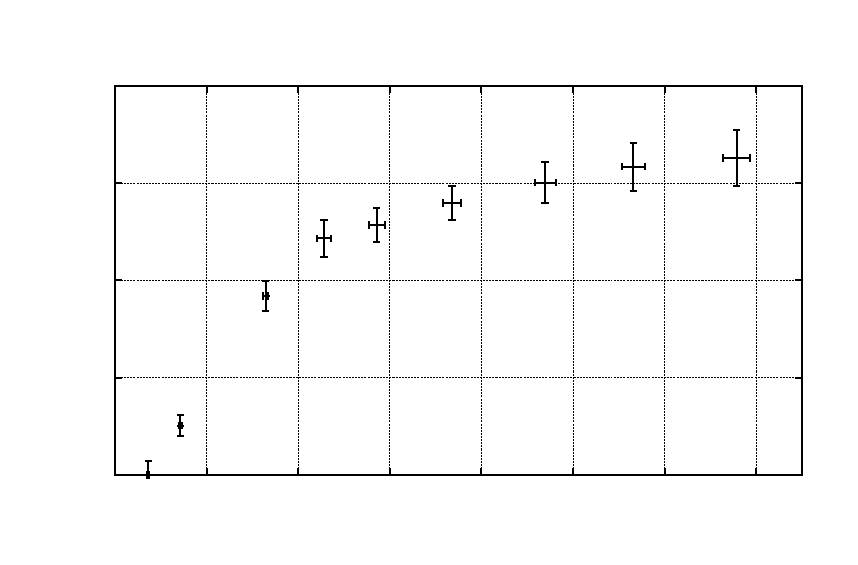
\includegraphics{hc1}}%
    \gplfronttext
  \end{picture}%
\endgroup

\caption{Koercivní síla kroužku I}
\label{g:hc1}
\end{graph}

\begin{graph}[htbp] 
\centering
% GNUPLOT: LaTeX picture with Postscript
\begingroup
  \makeatletter
  \providecommand\color[2][]{%
    \GenericError{(gnuplot) \space\space\space\@spaces}{%
      Package color not loaded in conjunction with
      terminal option `colourtext'%
    }{See the gnuplot documentation for explanation.%
    }{Either use 'blacktext' in gnuplot or load the package
      color.sty in LaTeX.}%
    \renewcommand\color[2][]{}%
  }%
  \providecommand\includegraphics[2][]{%
    \GenericError{(gnuplot) \space\space\space\@spaces}{%
      Package graphicx or graphics not loaded%
    }{See the gnuplot documentation for explanation.%
    }{The gnuplot epslatex terminal needs graphicx.sty or graphics.sty.}%
    \renewcommand\includegraphics[2][]{}%
  }%
  \providecommand\rotatebox[2]{#2}%
  \@ifundefined{ifGPcolor}{%
    \newif\ifGPcolor
    \GPcolorfalse
  }{}%
  \@ifundefined{ifGPblacktext}{%
    \newif\ifGPblacktext
    \GPblacktexttrue
  }{}%
  % define a \g@addto@macro without @ in the name:
  \let\gplgaddtomacro\g@addto@macro
  % define empty templates for all commands taking text:
  \gdef\gplbacktext{}%
  \gdef\gplfronttext{}%
  \makeatother
  \ifGPblacktext
    % no textcolor at all
    \def\colorrgb#1{}%
    \def\colorgray#1{}%
  \else
    % gray or color?
    \ifGPcolor
      \def\colorrgb#1{\color[rgb]{#1}}%
      \def\colorgray#1{\color[gray]{#1}}%
      \expandafter\def\csname LTw\endcsname{\color{white}}%
      \expandafter\def\csname LTb\endcsname{\color{black}}%
      \expandafter\def\csname LTa\endcsname{\color{black}}%
      \expandafter\def\csname LT0\endcsname{\color[rgb]{1,0,0}}%
      \expandafter\def\csname LT1\endcsname{\color[rgb]{0,1,0}}%
      \expandafter\def\csname LT2\endcsname{\color[rgb]{0,0,1}}%
      \expandafter\def\csname LT3\endcsname{\color[rgb]{1,0,1}}%
      \expandafter\def\csname LT4\endcsname{\color[rgb]{0,1,1}}%
      \expandafter\def\csname LT5\endcsname{\color[rgb]{1,1,0}}%
      \expandafter\def\csname LT6\endcsname{\color[rgb]{0,0,0}}%
      \expandafter\def\csname LT7\endcsname{\color[rgb]{1,0.3,0}}%
      \expandafter\def\csname LT8\endcsname{\color[rgb]{0.5,0.5,0.5}}%
    \else
      % gray
      \def\colorrgb#1{\color{black}}%
      \def\colorgray#1{\color[gray]{#1}}%
      \expandafter\def\csname LTw\endcsname{\color{white}}%
      \expandafter\def\csname LTb\endcsname{\color{black}}%
      \expandafter\def\csname LTa\endcsname{\color{black}}%
      \expandafter\def\csname LT0\endcsname{\color{black}}%
      \expandafter\def\csname LT1\endcsname{\color{black}}%
      \expandafter\def\csname LT2\endcsname{\color{black}}%
      \expandafter\def\csname LT3\endcsname{\color{black}}%
      \expandafter\def\csname LT4\endcsname{\color{black}}%
      \expandafter\def\csname LT5\endcsname{\color{black}}%
      \expandafter\def\csname LT6\endcsname{\color{black}}%
      \expandafter\def\csname LT7\endcsname{\color{black}}%
      \expandafter\def\csname LT8\endcsname{\color{black}}%
    \fi
  \fi
  \setlength{\unitlength}{0.0500bp}%
  \begin{picture}(7936.00,5102.00)%
    \gplgaddtomacro\gplbacktext{%
      \csname LTb\endcsname%
      \put(814,704){\makebox(0,0)[r]{\strut{} 0}}%
      \csname LTb\endcsname%
      \put(814,1383){\makebox(0,0)[r]{\strut{} 10}}%
      \csname LTb\endcsname%
      \put(814,2063){\makebox(0,0)[r]{\strut{} 20}}%
      \csname LTb\endcsname%
      \put(814,2742){\makebox(0,0)[r]{\strut{} 30}}%
      \csname LTb\endcsname%
      \put(814,3422){\makebox(0,0)[r]{\strut{} 40}}%
      \csname LTb\endcsname%
      \put(814,4101){\makebox(0,0)[r]{\strut{} 50}}%
      \csname LTb\endcsname%
      \put(946,484){\makebox(0,0){\strut{} 0}}%
      \csname LTb\endcsname%
      \put(2320,484){\makebox(0,0){\strut{} 50}}%
      \csname LTb\endcsname%
      \put(3693,484){\makebox(0,0){\strut{} 100}}%
      \csname LTb\endcsname%
      \put(5067,484){\makebox(0,0){\strut{} 150}}%
      \csname LTb\endcsname%
      \put(6440,484){\makebox(0,0){\strut{} 200}}%
      \put(176,2572){\rotatebox{-270}{\makebox(0,0){\strut{}$H_C$ (\si{\ampere\per\metre})}}}%
      \put(4242,154){\makebox(0,0){\strut{}$H_m$ (\si{\ampere\per\metre})}}%
      \put(4242,4771){\makebox(0,0){\strut{}Kroužek II - $H_C$}}%
    }%
    \gplgaddtomacro\gplfronttext{%
    }%
    \gplbacktext
    \put(0,0){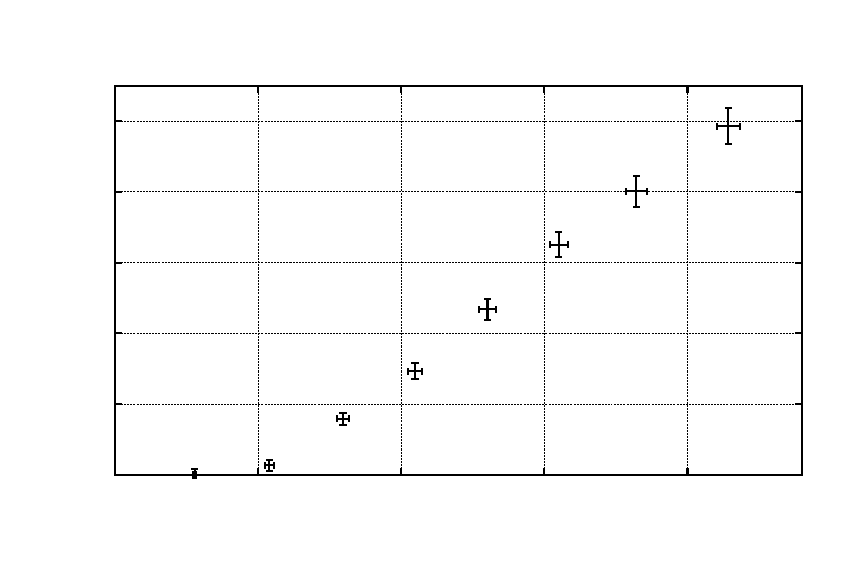
\includegraphics{hc2}}%
    \gplfronttext
  \end{picture}%
\endgroup

\caption{Koercivní síla kroužku II}
\label{g:hc2}
\end{graph}

\begin{graph}[htbp] 
\centering
% GNUPLOT: LaTeX picture with Postscript
\begingroup
  \makeatletter
  \providecommand\color[2][]{%
    \GenericError{(gnuplot) \space\space\space\@spaces}{%
      Package color not loaded in conjunction with
      terminal option `colourtext'%
    }{See the gnuplot documentation for explanation.%
    }{Either use 'blacktext' in gnuplot or load the package
      color.sty in LaTeX.}%
    \renewcommand\color[2][]{}%
  }%
  \providecommand\includegraphics[2][]{%
    \GenericError{(gnuplot) \space\space\space\@spaces}{%
      Package graphicx or graphics not loaded%
    }{See the gnuplot documentation for explanation.%
    }{The gnuplot epslatex terminal needs graphicx.sty or graphics.sty.}%
    \renewcommand\includegraphics[2][]{}%
  }%
  \providecommand\rotatebox[2]{#2}%
  \@ifundefined{ifGPcolor}{%
    \newif\ifGPcolor
    \GPcolorfalse
  }{}%
  \@ifundefined{ifGPblacktext}{%
    \newif\ifGPblacktext
    \GPblacktexttrue
  }{}%
  % define a \g@addto@macro without @ in the name:
  \let\gplgaddtomacro\g@addto@macro
  % define empty templates for all commands taking text:
  \gdef\gplbacktext{}%
  \gdef\gplfronttext{}%
  \makeatother
  \ifGPblacktext
    % no textcolor at all
    \def\colorrgb#1{}%
    \def\colorgray#1{}%
  \else
    % gray or color?
    \ifGPcolor
      \def\colorrgb#1{\color[rgb]{#1}}%
      \def\colorgray#1{\color[gray]{#1}}%
      \expandafter\def\csname LTw\endcsname{\color{white}}%
      \expandafter\def\csname LTb\endcsname{\color{black}}%
      \expandafter\def\csname LTa\endcsname{\color{black}}%
      \expandafter\def\csname LT0\endcsname{\color[rgb]{1,0,0}}%
      \expandafter\def\csname LT1\endcsname{\color[rgb]{0,1,0}}%
      \expandafter\def\csname LT2\endcsname{\color[rgb]{0,0,1}}%
      \expandafter\def\csname LT3\endcsname{\color[rgb]{1,0,1}}%
      \expandafter\def\csname LT4\endcsname{\color[rgb]{0,1,1}}%
      \expandafter\def\csname LT5\endcsname{\color[rgb]{1,1,0}}%
      \expandafter\def\csname LT6\endcsname{\color[rgb]{0,0,0}}%
      \expandafter\def\csname LT7\endcsname{\color[rgb]{1,0.3,0}}%
      \expandafter\def\csname LT8\endcsname{\color[rgb]{0.5,0.5,0.5}}%
    \else
      % gray
      \def\colorrgb#1{\color{black}}%
      \def\colorgray#1{\color[gray]{#1}}%
      \expandafter\def\csname LTw\endcsname{\color{white}}%
      \expandafter\def\csname LTb\endcsname{\color{black}}%
      \expandafter\def\csname LTa\endcsname{\color{black}}%
      \expandafter\def\csname LT0\endcsname{\color{black}}%
      \expandafter\def\csname LT1\endcsname{\color{black}}%
      \expandafter\def\csname LT2\endcsname{\color{black}}%
      \expandafter\def\csname LT3\endcsname{\color{black}}%
      \expandafter\def\csname LT4\endcsname{\color{black}}%
      \expandafter\def\csname LT5\endcsname{\color{black}}%
      \expandafter\def\csname LT6\endcsname{\color{black}}%
      \expandafter\def\csname LT7\endcsname{\color{black}}%
      \expandafter\def\csname LT8\endcsname{\color{black}}%
    \fi
  \fi
  \setlength{\unitlength}{0.0500bp}%
  \begin{picture}(7936.00,5102.00)%
    \gplgaddtomacro\gplbacktext{%
      \csname LTb\endcsname%
      \put(1078,704){\makebox(0,0)[r]{\strut{} 0}}%
      \csname LTb\endcsname%
      \put(1078,1594){\makebox(0,0)[r]{\strut{} 500}}%
      \csname LTb\endcsname%
      \put(1078,2484){\makebox(0,0)[r]{\strut{} 1000}}%
      \csname LTb\endcsname%
      \put(1078,3373){\makebox(0,0)[r]{\strut{} 1500}}%
      \csname LTb\endcsname%
      \put(1078,4263){\makebox(0,0)[r]{\strut{} 2000}}%
      \csname LTb\endcsname%
      \put(1210,484){\makebox(0,0){\strut{} 0}}%
      \csname LTb\endcsname%
      \put(2114,484){\makebox(0,0){\strut{} 1000}}%
      \csname LTb\endcsname%
      \put(3018,484){\makebox(0,0){\strut{} 2000}}%
      \csname LTb\endcsname%
      \put(3922,484){\makebox(0,0){\strut{} 3000}}%
      \csname LTb\endcsname%
      \put(4827,484){\makebox(0,0){\strut{} 4000}}%
      \csname LTb\endcsname%
      \put(5731,484){\makebox(0,0){\strut{} 5000}}%
      \csname LTb\endcsname%
      \put(6635,484){\makebox(0,0){\strut{} 6000}}%
      \csname LTb\endcsname%
      \put(7539,484){\makebox(0,0){\strut{} 7000}}%
      \put(176,2572){\rotatebox{-270}{\makebox(0,0){\strut{}$H_C$ (\si{\ampere\per\metre})}}}%
      \put(4374,154){\makebox(0,0){\strut{}$H_m$ (\si{\ampere\per\metre})}}%
      \put(4374,4771){\makebox(0,0){\strut{}Kroužek III - $H_C$}}%
    }%
    \gplgaddtomacro\gplfronttext{%
    }%
    \gplbacktext
    \put(0,0){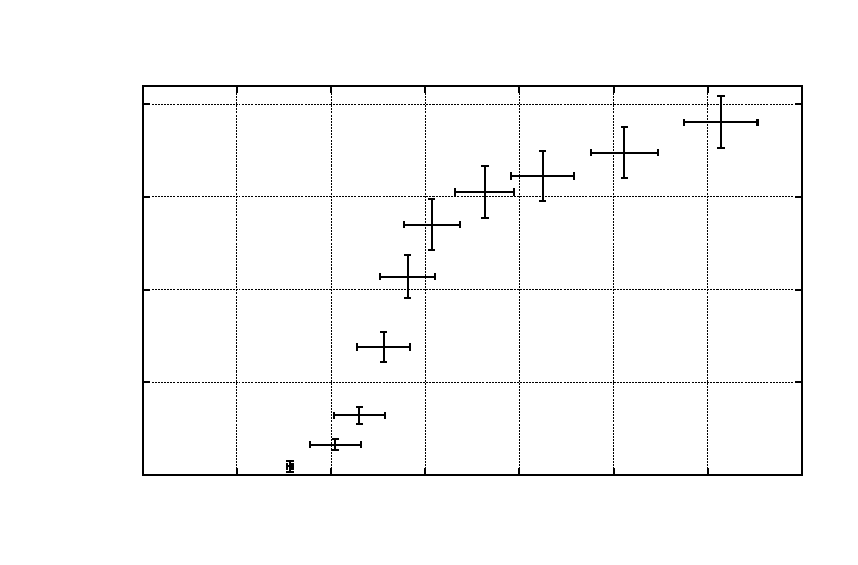
\includegraphics{hc3}}%
    \gplfronttext
  \end{picture}%
\endgroup

\caption{Koercivní síla kroužku III}
\label{g:hc3}
\end{graph}


\begin{graph}[htbp] 
\centering
% GNUPLOT: LaTeX picture with Postscript
\begingroup
  \makeatletter
  \providecommand\color[2][]{%
    \GenericError{(gnuplot) \space\space\space\@spaces}{%
      Package color not loaded in conjunction with
      terminal option `colourtext'%
    }{See the gnuplot documentation for explanation.%
    }{Either use 'blacktext' in gnuplot or load the package
      color.sty in LaTeX.}%
    \renewcommand\color[2][]{}%
  }%
  \providecommand\includegraphics[2][]{%
    \GenericError{(gnuplot) \space\space\space\@spaces}{%
      Package graphicx or graphics not loaded%
    }{See the gnuplot documentation for explanation.%
    }{The gnuplot epslatex terminal needs graphicx.sty or graphics.sty.}%
    \renewcommand\includegraphics[2][]{}%
  }%
  \providecommand\rotatebox[2]{#2}%
  \@ifundefined{ifGPcolor}{%
    \newif\ifGPcolor
    \GPcolorfalse
  }{}%
  \@ifundefined{ifGPblacktext}{%
    \newif\ifGPblacktext
    \GPblacktexttrue
  }{}%
  % define a \g@addto@macro without @ in the name:
  \let\gplgaddtomacro\g@addto@macro
  % define empty templates for all commands taking text:
  \gdef\gplbacktext{}%
  \gdef\gplfronttext{}%
  \makeatother
  \ifGPblacktext
    % no textcolor at all
    \def\colorrgb#1{}%
    \def\colorgray#1{}%
  \else
    % gray or color?
    \ifGPcolor
      \def\colorrgb#1{\color[rgb]{#1}}%
      \def\colorgray#1{\color[gray]{#1}}%
      \expandafter\def\csname LTw\endcsname{\color{white}}%
      \expandafter\def\csname LTb\endcsname{\color{black}}%
      \expandafter\def\csname LTa\endcsname{\color{black}}%
      \expandafter\def\csname LT0\endcsname{\color[rgb]{1,0,0}}%
      \expandafter\def\csname LT1\endcsname{\color[rgb]{0,1,0}}%
      \expandafter\def\csname LT2\endcsname{\color[rgb]{0,0,1}}%
      \expandafter\def\csname LT3\endcsname{\color[rgb]{1,0,1}}%
      \expandafter\def\csname LT4\endcsname{\color[rgb]{0,1,1}}%
      \expandafter\def\csname LT5\endcsname{\color[rgb]{1,1,0}}%
      \expandafter\def\csname LT6\endcsname{\color[rgb]{0,0,0}}%
      \expandafter\def\csname LT7\endcsname{\color[rgb]{1,0.3,0}}%
      \expandafter\def\csname LT8\endcsname{\color[rgb]{0.5,0.5,0.5}}%
    \else
      % gray
      \def\colorrgb#1{\color{black}}%
      \def\colorgray#1{\color[gray]{#1}}%
      \expandafter\def\csname LTw\endcsname{\color{white}}%
      \expandafter\def\csname LTb\endcsname{\color{black}}%
      \expandafter\def\csname LTa\endcsname{\color{black}}%
      \expandafter\def\csname LT0\endcsname{\color{black}}%
      \expandafter\def\csname LT1\endcsname{\color{black}}%
      \expandafter\def\csname LT2\endcsname{\color{black}}%
      \expandafter\def\csname LT3\endcsname{\color{black}}%
      \expandafter\def\csname LT4\endcsname{\color{black}}%
      \expandafter\def\csname LT5\endcsname{\color{black}}%
      \expandafter\def\csname LT6\endcsname{\color{black}}%
      \expandafter\def\csname LT7\endcsname{\color{black}}%
      \expandafter\def\csname LT8\endcsname{\color{black}}%
    \fi
  \fi
  \setlength{\unitlength}{0.0500bp}%
  \begin{picture}(7936.00,5102.00)%
    \gplgaddtomacro\gplbacktext{%
      \csname LTb\endcsname%
      \put(1078,704){\makebox(0,0)[r]{\strut{} 0}}%
      \csname LTb\endcsname%
      \put(1078,1327){\makebox(0,0)[r]{\strut{} 0.05}}%
      \csname LTb\endcsname%
      \put(1078,1950){\makebox(0,0)[r]{\strut{} 0.1}}%
      \csname LTb\endcsname%
      \put(1078,2573){\makebox(0,0)[r]{\strut{} 0.15}}%
      \csname LTb\endcsname%
      \put(1078,3195){\makebox(0,0)[r]{\strut{} 0.2}}%
      \csname LTb\endcsname%
      \put(1078,3818){\makebox(0,0)[r]{\strut{} 0.25}}%
      \csname LTb\endcsname%
      \put(1078,4441){\makebox(0,0)[r]{\strut{} 0.3}}%
      \csname LTb\endcsname%
      \put(1210,484){\makebox(0,0){\strut{} 0}}%
      \csname LTb\endcsname%
      \put(2054,484){\makebox(0,0){\strut{} 20}}%
      \csname LTb\endcsname%
      \put(2898,484){\makebox(0,0){\strut{} 40}}%
      \csname LTb\endcsname%
      \put(3742,484){\makebox(0,0){\strut{} 60}}%
      \csname LTb\endcsname%
      \put(4585,484){\makebox(0,0){\strut{} 80}}%
      \csname LTb\endcsname%
      \put(5429,484){\makebox(0,0){\strut{} 100}}%
      \csname LTb\endcsname%
      \put(6273,484){\makebox(0,0){\strut{} 120}}%
      \csname LTb\endcsname%
      \put(7117,484){\makebox(0,0){\strut{} 140}}%
      \put(176,2572){\rotatebox{-270}{\makebox(0,0){\strut{}$B_m$ (\si{\tesla})}}}%
      \put(4374,154){\makebox(0,0){\strut{}$H_m$ (\si{\ampere\per\metre})}}%
      \put(4374,4771){\makebox(0,0){\strut{}Kroužek I - $B_m$}}%
    }%
    \gplgaddtomacro\gplfronttext{%
    }%
    \gplbacktext
    \put(0,0){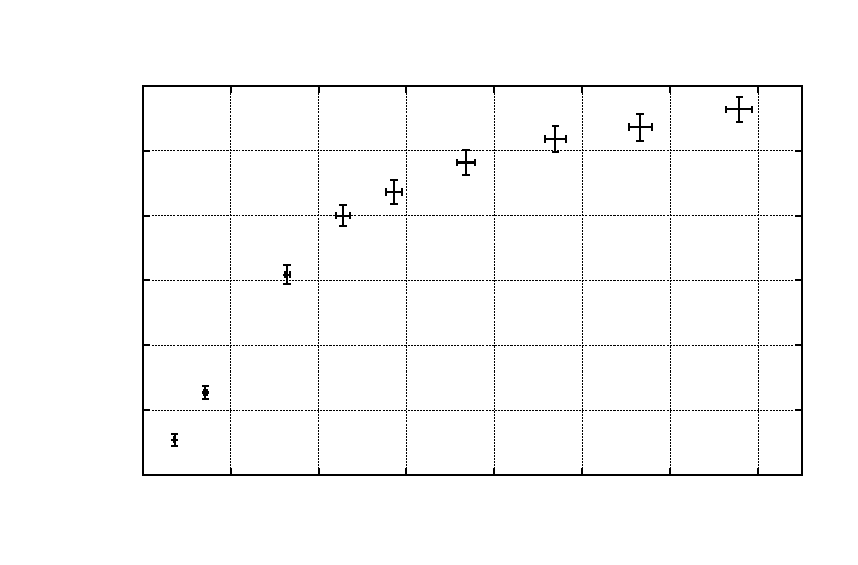
\includegraphics{bm1}}%
    \gplfronttext
  \end{picture}%
\endgroup

\caption{Magnetická indukce v kroužku I}
\label{g:bm1}
\end{graph}

\begin{graph}[htbp] 
\centering
% GNUPLOT: LaTeX picture with Postscript
\begingroup
  \makeatletter
  \providecommand\color[2][]{%
    \GenericError{(gnuplot) \space\space\space\@spaces}{%
      Package color not loaded in conjunction with
      terminal option `colourtext'%
    }{See the gnuplot documentation for explanation.%
    }{Either use 'blacktext' in gnuplot or load the package
      color.sty in LaTeX.}%
    \renewcommand\color[2][]{}%
  }%
  \providecommand\includegraphics[2][]{%
    \GenericError{(gnuplot) \space\space\space\@spaces}{%
      Package graphicx or graphics not loaded%
    }{See the gnuplot documentation for explanation.%
    }{The gnuplot epslatex terminal needs graphicx.sty or graphics.sty.}%
    \renewcommand\includegraphics[2][]{}%
  }%
  \providecommand\rotatebox[2]{#2}%
  \@ifundefined{ifGPcolor}{%
    \newif\ifGPcolor
    \GPcolorfalse
  }{}%
  \@ifundefined{ifGPblacktext}{%
    \newif\ifGPblacktext
    \GPblacktexttrue
  }{}%
  % define a \g@addto@macro without @ in the name:
  \let\gplgaddtomacro\g@addto@macro
  % define empty templates for all commands taking text:
  \gdef\gplbacktext{}%
  \gdef\gplfronttext{}%
  \makeatother
  \ifGPblacktext
    % no textcolor at all
    \def\colorrgb#1{}%
    \def\colorgray#1{}%
  \else
    % gray or color?
    \ifGPcolor
      \def\colorrgb#1{\color[rgb]{#1}}%
      \def\colorgray#1{\color[gray]{#1}}%
      \expandafter\def\csname LTw\endcsname{\color{white}}%
      \expandafter\def\csname LTb\endcsname{\color{black}}%
      \expandafter\def\csname LTa\endcsname{\color{black}}%
      \expandafter\def\csname LT0\endcsname{\color[rgb]{1,0,0}}%
      \expandafter\def\csname LT1\endcsname{\color[rgb]{0,1,0}}%
      \expandafter\def\csname LT2\endcsname{\color[rgb]{0,0,1}}%
      \expandafter\def\csname LT3\endcsname{\color[rgb]{1,0,1}}%
      \expandafter\def\csname LT4\endcsname{\color[rgb]{0,1,1}}%
      \expandafter\def\csname LT5\endcsname{\color[rgb]{1,1,0}}%
      \expandafter\def\csname LT6\endcsname{\color[rgb]{0,0,0}}%
      \expandafter\def\csname LT7\endcsname{\color[rgb]{1,0.3,0}}%
      \expandafter\def\csname LT8\endcsname{\color[rgb]{0.5,0.5,0.5}}%
    \else
      % gray
      \def\colorrgb#1{\color{black}}%
      \def\colorgray#1{\color[gray]{#1}}%
      \expandafter\def\csname LTw\endcsname{\color{white}}%
      \expandafter\def\csname LTb\endcsname{\color{black}}%
      \expandafter\def\csname LTa\endcsname{\color{black}}%
      \expandafter\def\csname LT0\endcsname{\color{black}}%
      \expandafter\def\csname LT1\endcsname{\color{black}}%
      \expandafter\def\csname LT2\endcsname{\color{black}}%
      \expandafter\def\csname LT3\endcsname{\color{black}}%
      \expandafter\def\csname LT4\endcsname{\color{black}}%
      \expandafter\def\csname LT5\endcsname{\color{black}}%
      \expandafter\def\csname LT6\endcsname{\color{black}}%
      \expandafter\def\csname LT7\endcsname{\color{black}}%
      \expandafter\def\csname LT8\endcsname{\color{black}}%
    \fi
  \fi
  \setlength{\unitlength}{0.0500bp}%
  \begin{picture}(7936.00,5102.00)%
    \gplgaddtomacro\gplbacktext{%
      \csname LTb\endcsname%
      \put(1078,704){\makebox(0,0)[r]{\strut{} 0}}%
      \csname LTb\endcsname%
      \put(1078,1451){\makebox(0,0)[r]{\strut{} 0.05}}%
      \csname LTb\endcsname%
      \put(1078,2199){\makebox(0,0)[r]{\strut{} 0.1}}%
      \csname LTb\endcsname%
      \put(1078,2946){\makebox(0,0)[r]{\strut{} 0.15}}%
      \csname LTb\endcsname%
      \put(1078,3694){\makebox(0,0)[r]{\strut{} 0.2}}%
      \csname LTb\endcsname%
      \put(1078,4441){\makebox(0,0)[r]{\strut{} 0.25}}%
      \csname LTb\endcsname%
      \put(1210,484){\makebox(0,0){\strut{} 0}}%
      \csname LTb\endcsname%
      \put(2529,484){\makebox(0,0){\strut{} 50}}%
      \csname LTb\endcsname%
      \put(3847,484){\makebox(0,0){\strut{} 100}}%
      \csname LTb\endcsname%
      \put(5166,484){\makebox(0,0){\strut{} 150}}%
      \csname LTb\endcsname%
      \put(6484,484){\makebox(0,0){\strut{} 200}}%
      \put(176,2572){\rotatebox{-270}{\makebox(0,0){\strut{}$B_m$ (\si{\tesla})}}}%
      \put(4374,154){\makebox(0,0){\strut{}$H_m$ (\si{\ampere\per\metre})}}%
      \put(4374,4771){\makebox(0,0){\strut{}Kroužek II - $B_m$}}%
    }%
    \gplgaddtomacro\gplfronttext{%
    }%
    \gplbacktext
    \put(0,0){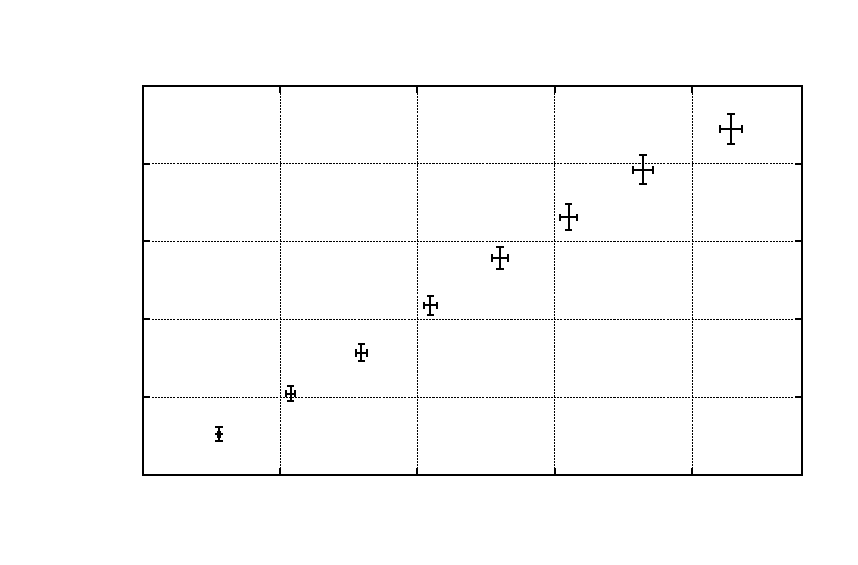
\includegraphics{bm2}}%
    \gplfronttext
  \end{picture}%
\endgroup

\caption{Magnetická indukce v kroužku II}
\label{g:bm2}
\end{graph}

\begin{graph}[htbp] 
\centering
% GNUPLOT: LaTeX picture with Postscript
\begingroup
  \makeatletter
  \providecommand\color[2][]{%
    \GenericError{(gnuplot) \space\space\space\@spaces}{%
      Package color not loaded in conjunction with
      terminal option `colourtext'%
    }{See the gnuplot documentation for explanation.%
    }{Either use 'blacktext' in gnuplot or load the package
      color.sty in LaTeX.}%
    \renewcommand\color[2][]{}%
  }%
  \providecommand\includegraphics[2][]{%
    \GenericError{(gnuplot) \space\space\space\@spaces}{%
      Package graphicx or graphics not loaded%
    }{See the gnuplot documentation for explanation.%
    }{The gnuplot epslatex terminal needs graphicx.sty or graphics.sty.}%
    \renewcommand\includegraphics[2][]{}%
  }%
  \providecommand\rotatebox[2]{#2}%
  \@ifundefined{ifGPcolor}{%
    \newif\ifGPcolor
    \GPcolorfalse
  }{}%
  \@ifundefined{ifGPblacktext}{%
    \newif\ifGPblacktext
    \GPblacktexttrue
  }{}%
  % define a \g@addto@macro without @ in the name:
  \let\gplgaddtomacro\g@addto@macro
  % define empty templates for all commands taking text:
  \gdef\gplbacktext{}%
  \gdef\gplfronttext{}%
  \makeatother
  \ifGPblacktext
    % no textcolor at all
    \def\colorrgb#1{}%
    \def\colorgray#1{}%
  \else
    % gray or color?
    \ifGPcolor
      \def\colorrgb#1{\color[rgb]{#1}}%
      \def\colorgray#1{\color[gray]{#1}}%
      \expandafter\def\csname LTw\endcsname{\color{white}}%
      \expandafter\def\csname LTb\endcsname{\color{black}}%
      \expandafter\def\csname LTa\endcsname{\color{black}}%
      \expandafter\def\csname LT0\endcsname{\color[rgb]{1,0,0}}%
      \expandafter\def\csname LT1\endcsname{\color[rgb]{0,1,0}}%
      \expandafter\def\csname LT2\endcsname{\color[rgb]{0,0,1}}%
      \expandafter\def\csname LT3\endcsname{\color[rgb]{1,0,1}}%
      \expandafter\def\csname LT4\endcsname{\color[rgb]{0,1,1}}%
      \expandafter\def\csname LT5\endcsname{\color[rgb]{1,1,0}}%
      \expandafter\def\csname LT6\endcsname{\color[rgb]{0,0,0}}%
      \expandafter\def\csname LT7\endcsname{\color[rgb]{1,0.3,0}}%
      \expandafter\def\csname LT8\endcsname{\color[rgb]{0.5,0.5,0.5}}%
    \else
      % gray
      \def\colorrgb#1{\color{black}}%
      \def\colorgray#1{\color[gray]{#1}}%
      \expandafter\def\csname LTw\endcsname{\color{white}}%
      \expandafter\def\csname LTb\endcsname{\color{black}}%
      \expandafter\def\csname LTa\endcsname{\color{black}}%
      \expandafter\def\csname LT0\endcsname{\color{black}}%
      \expandafter\def\csname LT1\endcsname{\color{black}}%
      \expandafter\def\csname LT2\endcsname{\color{black}}%
      \expandafter\def\csname LT3\endcsname{\color{black}}%
      \expandafter\def\csname LT4\endcsname{\color{black}}%
      \expandafter\def\csname LT5\endcsname{\color{black}}%
      \expandafter\def\csname LT6\endcsname{\color{black}}%
      \expandafter\def\csname LT7\endcsname{\color{black}}%
      \expandafter\def\csname LT8\endcsname{\color{black}}%
    \fi
  \fi
  \setlength{\unitlength}{0.0500bp}%
  \begin{picture}(7936.00,5102.00)%
    \gplgaddtomacro\gplbacktext{%
      \csname LTb\endcsname%
      \put(1078,704){\makebox(0,0)[r]{\strut{} 0}}%
      \csname LTb\endcsname%
      \put(1078,1327){\makebox(0,0)[r]{\strut{} 0.05}}%
      \csname LTb\endcsname%
      \put(1078,1950){\makebox(0,0)[r]{\strut{} 0.1}}%
      \csname LTb\endcsname%
      \put(1078,2573){\makebox(0,0)[r]{\strut{} 0.15}}%
      \csname LTb\endcsname%
      \put(1078,3195){\makebox(0,0)[r]{\strut{} 0.2}}%
      \csname LTb\endcsname%
      \put(1078,3818){\makebox(0,0)[r]{\strut{} 0.25}}%
      \csname LTb\endcsname%
      \put(1078,4441){\makebox(0,0)[r]{\strut{} 0.3}}%
      \csname LTb\endcsname%
      \put(1210,484){\makebox(0,0){\strut{} 0}}%
      \csname LTb\endcsname%
      \put(2114,484){\makebox(0,0){\strut{} 1000}}%
      \csname LTb\endcsname%
      \put(3018,484){\makebox(0,0){\strut{} 2000}}%
      \csname LTb\endcsname%
      \put(3922,484){\makebox(0,0){\strut{} 3000}}%
      \csname LTb\endcsname%
      \put(4827,484){\makebox(0,0){\strut{} 4000}}%
      \csname LTb\endcsname%
      \put(5731,484){\makebox(0,0){\strut{} 5000}}%
      \csname LTb\endcsname%
      \put(6635,484){\makebox(0,0){\strut{} 6000}}%
      \csname LTb\endcsname%
      \put(7539,484){\makebox(0,0){\strut{} 7000}}%
      \put(176,2572){\rotatebox{-270}{\makebox(0,0){\strut{}$B_m$ (\si{\tesla})}}}%
      \put(4374,154){\makebox(0,0){\strut{}$H_m$ (\si{\ampere\per\metre})}}%
      \put(4374,4771){\makebox(0,0){\strut{}Kroužek III - $B_m$}}%
    }%
    \gplgaddtomacro\gplfronttext{%
    }%
    \gplbacktext
    \put(0,0){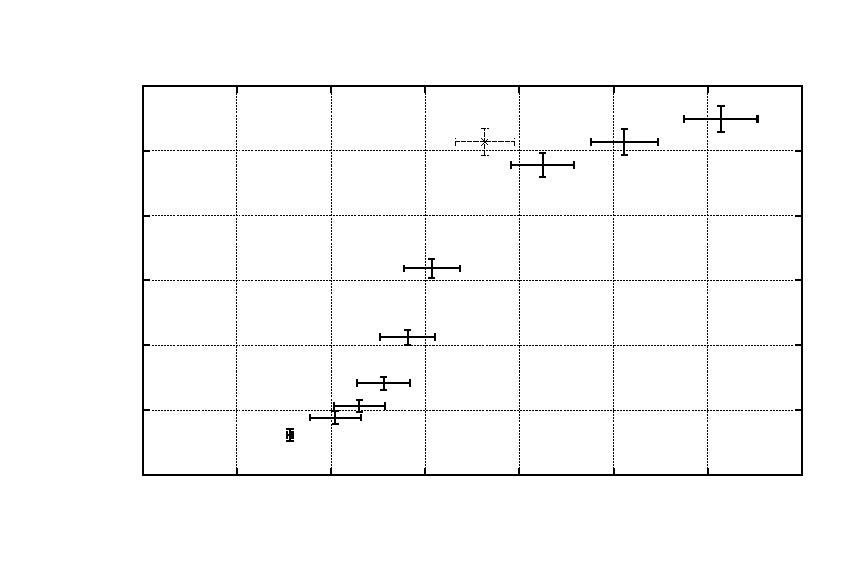
\includegraphics{bm3}}%
    \gplfronttext
  \end{picture}%
\endgroup

\caption{Magnetická indukce v kroužku III, bod slabou čarou ($H_C=\SI{3630}{\ampere\per\metre}$) je pravděpodobně hrubá chyba}
\label{g:bm3}
\end{graph}

Hysterezní smyčka měla tvar úsečky u kroužku I přibližně do \SI{8}{\ampere\per\metre}, u kroužku II do \SI{50}{\ampere\per\metre} a u kroužku III do \SI{2000}{\ampere\per\metre}.
Při vyšších intenzitách pole se už začaly uplatňovat nevratné děje a smyčka měla Rayleighův tvar.
Smyčka přešla v normální tvar u kroužku I přibližně při \SI{15}{\ampere\per\metre} a u kroužku II při \SI{100}{\ampere\per\metre}
U kroužku III měla smyčka v Rayleighově oblasti přiškrcený tvar, do normálního tvaru přešla přibližně při \SI{5000}{\ampere\per\metre}.